In this chapter we will briefly describe electronic voting in general, focusing mostly on the challenges and security parameters.

\section{Introduction}
In many aspects of our life's we in counter the act of voting, from simple things as voting whats for dinner, to the more complex things as a government election. The later involving a large number of people from different geographical locations. These election is normally handled by dividing the people into sections based on location, each section handling it's own sub-election and submitting the result to a overall tally. Though many countries still mostly rely on the old fashioned paper based ballots, we have in the recent years seen an increase in electronic voting. Electronic voting refers to the act of voting though an electronic devices and depending on the voting equipment and location, it can be divide into five categories \cite{Cet09}. 

\section{Classification}

\begin{description}
\item[DRE voting] Direct Recording Electronic is a specialized standalone electronic voting machine, which have the attributes of being physically hardened and have software specifically for voting installed. Votes casted on a DRE is do within a voting booth located on a polling site, and the votes is then recorded into a electronic ballot box.

\item[Poll-site voting] The voting is located on a polling site, votes are cast on public computers located on the site, in favour for voting booths. The computers on site are connected to a counting authority server though a closed and controlled network. Authentication can be done prior to the voting period or at the polling site

\item[Poll-site kiosk voting] Votes are casted inside a voting booth located at a polling site, using a terminal. The terminal is connected to a counting authority server though a closed and controlled network. Authentication is done at the polling site before allowed access to the voting booth. 

\item[Poll-site Internet voting] Votes are casted on public computers located on a polling site. The public computers on site is online and connected to a counting authority server over uncontrolled network. Authentication can be done prior to the voting period or at the polling site

\item[Remote Internet voting] Simply requires internet access and can be done from a home computer. Authentication is done prior to the voting an typical involves password or some type of authentication token. 

\end{description}


\section{The Voting Process}
Similar to the classification, there exist several of different systems and protocols for voting. But they typically all follows the same process and includes the same actors as illustrated and describe below \cite{Cet09}. 

\begin{figure}[H]
\centering
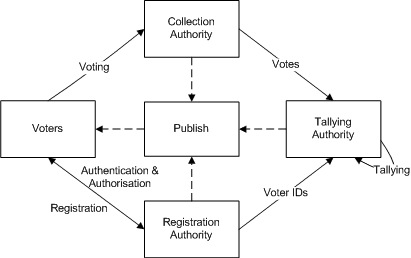
\includegraphics[scale=0.7]{Voting_Process.png}

\caption{Voting process}
\label{fig:Voting_Process}
\end{figure}

\begin{description}
    \item[Voter] A registered voter that has the right to cast a vote in the election.  
    
    \item[Registration authority] Registration authority is responsible for registering eligible voters, and ensuring that
    only these voters are allowed to vote, and only votes ones. 
        
    \item[Collection authority] The collection authority are responsible for collecting all the votes

    \item[Tallying authority] Tallying authority are responsible for counting the votes of the election and publishing the result. 
\end{description}


\noindent
The voting process as illustrated on figure \ref{fig:Voting_Process} holds true for any voting system, and includes four stages. 

\begin{description}
    \item[Registration] Prior to the election eligible voters registers to vote in the election. 
    
    \item[Authentication and Authorisation] Registered voters are authenticated, if they are found eligible and have not voted yet, and are giving the privileges of voting to the election. 
        
    \item[Voting] The voters cast there votes. 

    \item[Tallying] The Tallying authority counts the votes and publishes the result. 
\end{description}


\section{Challenges}
Though the voting process and actors is basically similar for any voting system, electronic or not. 


In their paper Damgård, Groth and Gorm outline three important challenges
that need to be solved [DGS02]:

\begin{description}
    \item[Privacy] Only the final result should be made public, no information
        about the votes must be leaked.

    \item[Robustness] The result will reflect all submitted and well-formed ballots
        correctly, even if some voters or entities running the election cheat.

    \item[Universal verifiability] After the election, the result can be verified by
        anyone. In order words, any party should be able to convince himself
        that the election was fair in the sense that the published tally was
        correctly computed.
\end{description}


\section{Security Requirements}

\cite{Cet08}
\begin{itemize}
    \item \textit{Voter Privacy}
        No one should be able to link a vote back to the specific voter, and only the voter should
        know his vote. These requirements shall hold during and after the election.  
    
    \item \textit{Eligibility}    
        Only Eligible and registered voters can vote. 
    
    \item \textit{Uniqueness}
        Only one vote per registered voter should be counted.
    
    \item \textit{Fairness}
        None should be able to gain any knowledge of the outcome of the election, before the ending. This is to prevent voters of voting accordingly to any leaked information. 
    
    \item \textit{Uncoercibility}
        Nobody should be able to extract the value of a vote. This is to prevent anybody from compelling a voter by force, intimidation, or authority to cast a vote in a specific way. 
    
    \item \textit{Receipt-freeness} 
        The voting system should not produce a receipt that reveals any information about the casted vote. This is to prevent a vote from trading his vote. 
    
    \item \textit{Accuracy} 
        The final tally should be correctly computed from valid casted votes. It should not be
        possible to manipulate the final tally without being detected. 
    
    \item \textit{Universal Verifiability}
        It should be possible for any participants and observers to validate individual votes as well as the final tally of the election. 
    
    \item \textit{Individual Verifiability}    
        Every registered voter should be able to verify that his vote is counted correctly. 
    
\end{itemize}

\section{Approaches}

\begin{description}
    \item[Mix-nets] In mix-net voting schemes, the ballots of all voters are shuffled through a
        mix-net, such that afterwards, it is unclear which ballot belongs to which
        voter. More precisely, the voter encrypts his vote consecutively with the
        public key of each mixer, then all these multi-encrypted votes are sequentially
        decrypted and permuted by each mixer. The output of the
        last mixer is a shuffle of the votes in clear, but in random order. These
        votes can then be tallied publicly. In order to guarantee correctness of the
        tally, every mixer must additional publish a proof that he did not modify
        or substitute votes. This process is illustrated in Figure 1.2.
        For the first mixer, the secrecy of the votes is based on the infeasibility
        of decrypting, and with each mixer, the level of encryption is decreased,
        but the level of anonymity of the voter is increased. The correctness is
        22 Introduction
        based on the soundness of the public proofs. Because at the end all votes
        are known in clear, invalid votes can be discarded easily.
    
    
    \item[Blind signatures] This approach can be seen as an abstraction of mix-net voting            schemes. Here, each voter casts his vote unencrypted, but anonymously. The security
        of this scheme is based on hiding which vote belongs to which voter.
        Additional efforts are needed to ensure that only entitled voters can cast
        a vote: Each voter is to get a blindly signed public key from a registration
        authority, with which he signs his vote and sends it over an anonymous
        channel to the bulletin board. This approach is illustrated in Figure 1.3.
        
        
    \item[Homomorphic encryption] A homomorphic encryption scheme supports addition of               ciphertexts without knowledge of the secret key. With this primitive, one can construct
        very efficient voting protocols: The voter encrypts his vote with a
        homomorphic encryption scheme and posts it to the bulletin board. The
        authorities can tally the encrypted votes and decrypt the sum (see Figure
        1.4). In addition, each voter must prove the validity of the submitted
        vote. In this approach, it is clear which (encrypted) vote belongs to which
        voter, and the secrecy of the votes is based on the infeasibility of decrypting
        votes.
\end{description}


\begin{description}
    \item[Voter]
    \item[Tallier]
    \item[Observer]
    \item[Bulletin board]
\end{description}